\documentclass{standalone}
\usepackage{tikz}
\usetikzlibrary{patterns, positioning}
\usepackage[sfdefault]{ClearSans} %% option 'sfdefault' activates Clear Sans as the default text font
\usepackage[T1]{fontenc}

\begin{document}
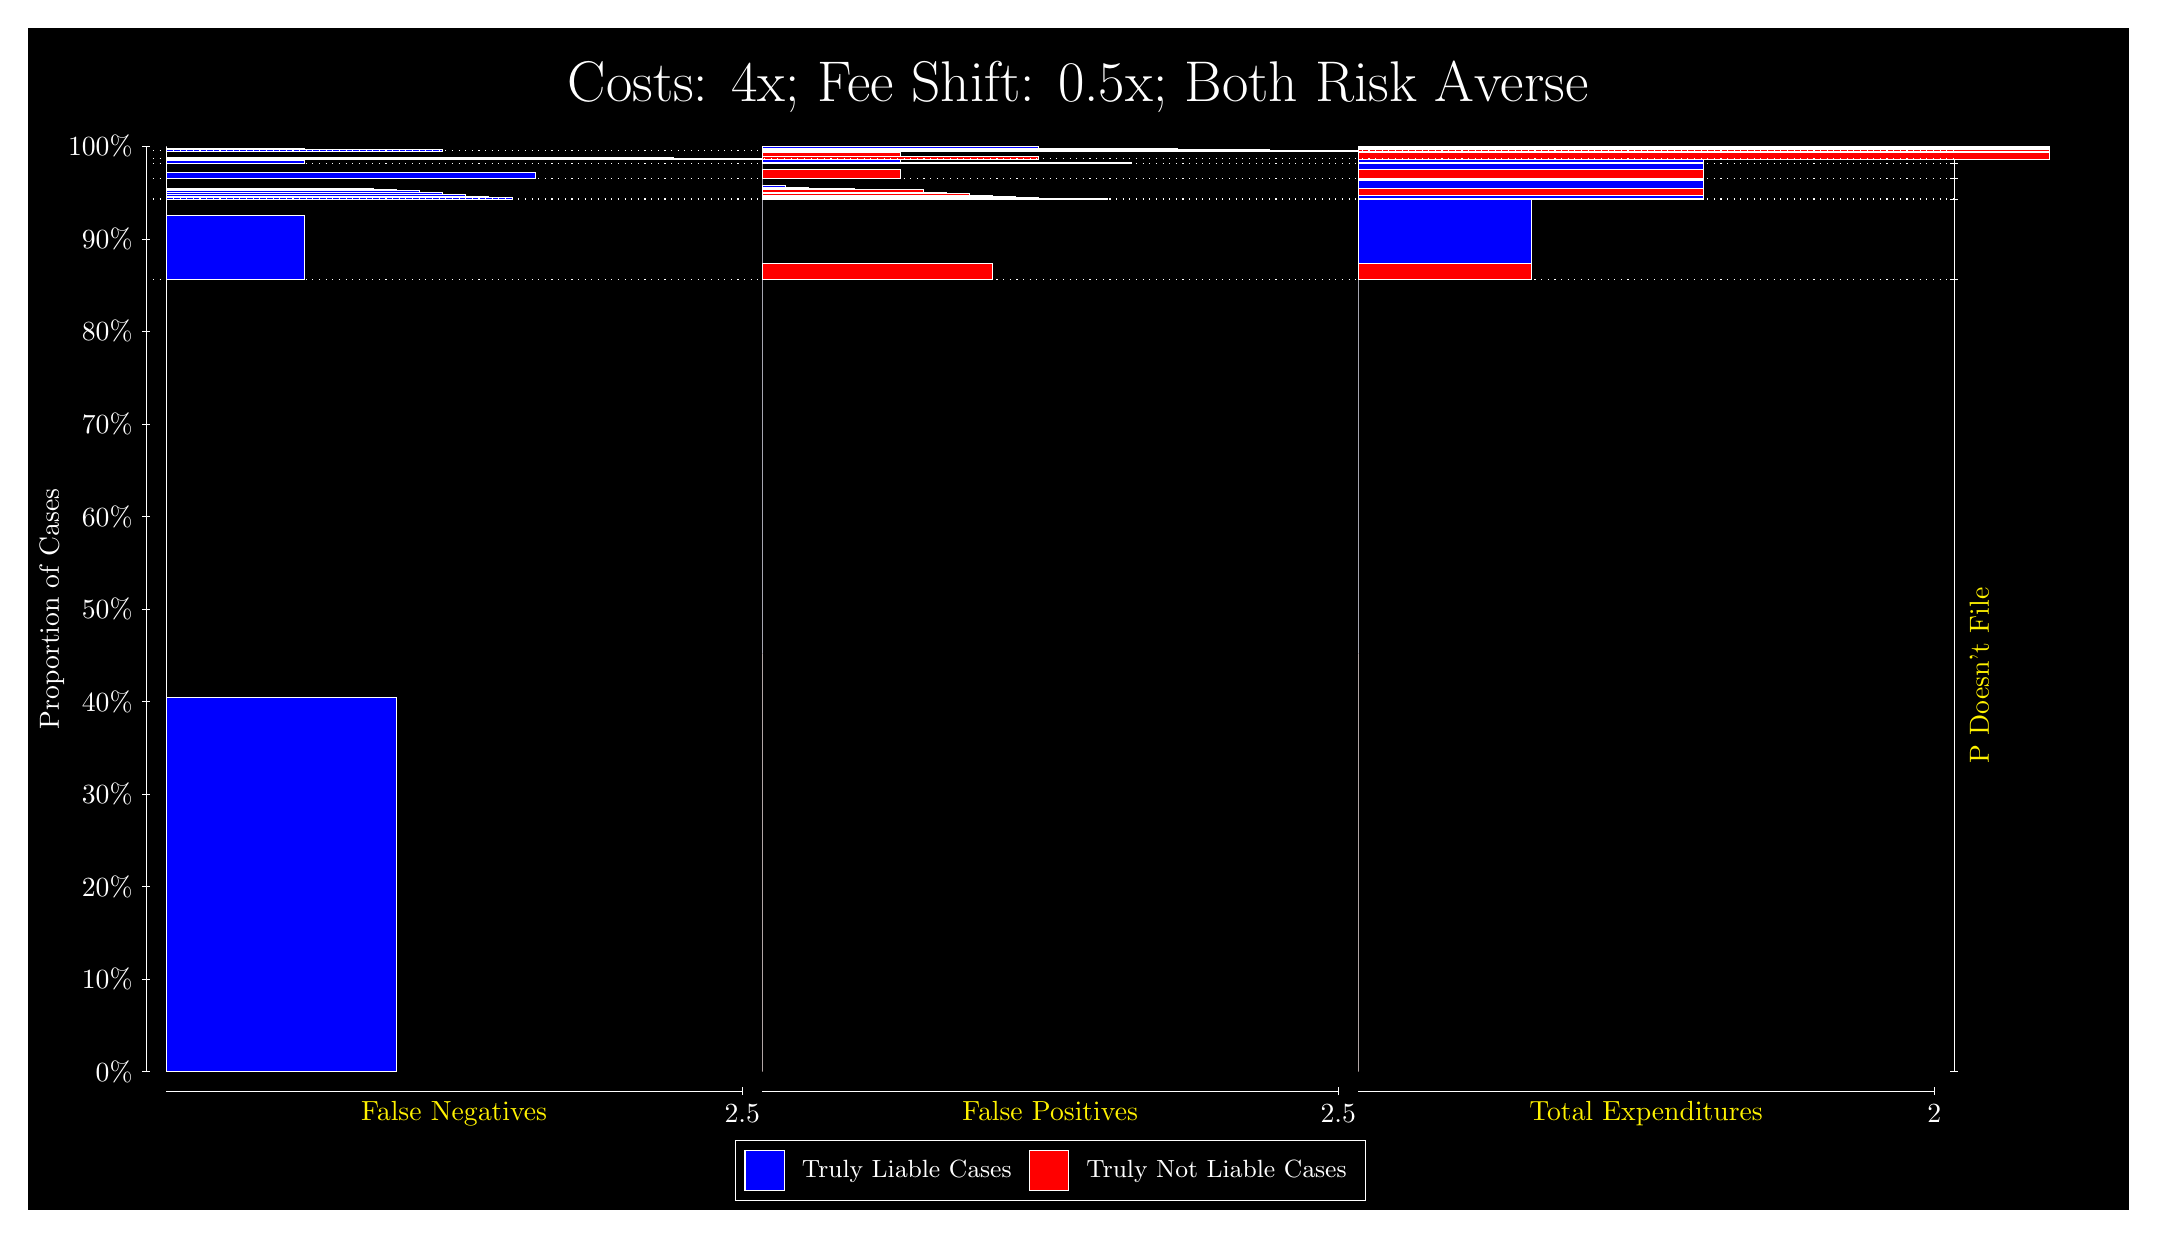
\begin{tikzpicture}
\draw[fill=black] (0,0) rectangle (26.667,15);
\draw[text=white] (0,13.5) rectangle (26.667,15) node[midway] {\huge Costs: 4x; Fee Shift: 0.5x; Both Risk Averse};
\draw[white, very thin] (1.5,1.75) -- (1.5,13.5);
\node[rotate=90, text=white, anchor=center] at (0.3, 7.625) {Proportion of Cases};
\draw[white, very thin] (1.45,1.75) -- (1.55,1.75);
\node[text=white, anchor=east] at (1.45, 1.75) {0\%};
\draw[white, very thin] (1.45,2.925) -- (1.55,2.925);
\node[text=white, anchor=east] at (1.45, 2.925) {10\%};
\draw[white, very thin] (1.45,4.1) -- (1.55,4.1);
\node[text=white, anchor=east] at (1.45, 4.1) {20\%};
\draw[white, very thin] (1.45,5.275) -- (1.55,5.275);
\node[text=white, anchor=east] at (1.45, 5.275) {30\%};
\draw[white, very thin] (1.45,6.45) -- (1.55,6.45);
\node[text=white, anchor=east] at (1.45, 6.45) {40\%};
\draw[white, very thin] (1.45,7.625) -- (1.55,7.625);
\node[text=white, anchor=east] at (1.45, 7.625) {50\%};
\draw[white, very thin] (1.45,8.8) -- (1.55,8.8);
\node[text=white, anchor=east] at (1.45, 8.8) {60\%};
\draw[white, very thin] (1.45,9.975) -- (1.55,9.975);
\node[text=white, anchor=east] at (1.45, 9.975) {70\%};
\draw[white, very thin] (1.45,11.15) -- (1.55,11.15);
\node[text=white, anchor=east] at (1.45, 11.15) {80\%};
\draw[white, very thin] (1.45,12.325) -- (1.55,12.325);
\node[text=white, anchor=east] at (1.45, 12.325) {90\%};
\draw[white, very thin] (1.45,13.5) -- (1.55,13.5);
\node[text=white, anchor=east] at (1.45, 13.5) {100\%};

\draw[white, very thin] (24.457,1.75) -- (24.457,13.5);
\draw[white, very thin] (24.407,1.75) -- (24.507,1.75);
\node[anchor=west] at (24.407, 1.75) {};
\draw[white, very thin] (24.407,11.808) -- (24.507,11.808);
\node[anchor=west] at (24.407, 11.808) {};
\draw[white, very thin] (24.407,12.831) -- (24.507,12.831);
\node[anchor=west] at (24.407, 12.831) {};
\draw[white, very thin] (24.407,13.093) -- (24.507,13.093);
\node[anchor=west] at (24.407, 13.093) {};
\draw[white, very thin] (24.407,13.283) -- (24.507,13.283);
\node[anchor=west] at (24.407, 13.283) {};
\draw[white, very thin] (24.407,13.341) -- (24.507,13.341);
\node[anchor=west] at (24.407, 13.341) {};
\draw[white, very thin] (24.407,13.442) -- (24.507,13.442);
\node[anchor=west] at (24.407, 13.442) {};
\draw[white, very thin] (24.407,13.5) -- (24.507,13.5);
\node[anchor=west] at (24.407, 13.5) {};

\draw[white, very thin, fill=blue] (1.75,1.75) rectangle (4.6775,6.4982);
\draw[white, very thin, fill=red] (1.75,6.4982) rectangle (1.75,11.808);
\draw[white, very thin, fill=blue] (1.75,11.808) rectangle (3.5065,12.623);
\draw[white, very thin, fill=red] (1.75,12.623) rectangle (1.75,12.831);
\draw[white, very thin, fill=blue] (1.75,12.831) rectangle (6.1413,12.853);
\draw[white, very thin, fill=blue] (1.75,12.853) rectangle (5.8486,12.86);
\draw[white, very thin, fill=blue] (1.75,12.86) rectangle (5.5558,12.887);
\draw[white, very thin, fill=blue] (1.75,12.887) rectangle (5.2631,12.916);
\draw[white, very thin, fill=blue] (1.75,12.916) rectangle (4.9703,12.945);
\draw[white, very thin, fill=blue] (1.75,12.945) rectangle (4.6775,12.954);
\draw[white, very thin, fill=blue] (1.75,12.954) rectangle (4.3848,12.962);
\draw[white, very thin, fill=blue] (1.75,12.962) rectangle (4.092,12.966);
\draw[white, very thin, fill=blue] (1.75,12.966) rectangle (3.7993,12.97);
\draw[white, very thin, fill=red] (1.75,12.97) rectangle (1.75,13.093);
\draw[white, very thin, fill=blue] (1.75,13.093) rectangle (6.4341,13.166);
\draw[white, very thin, fill=red] (1.75,13.166) rectangle (1.75,13.283);
\draw[white, very thin, fill=blue] (1.75,13.283) rectangle (3.5065,13.325);
\draw[white, very thin, fill=red] (1.75,13.325) rectangle (1.75,13.341);
\draw[white, very thin, fill=blue] (1.75,13.341) rectangle (9.9471,13.347);
\draw[white, very thin, fill=blue] (1.75,13.347) rectangle (8.1906,13.36);
\draw[white, very thin, fill=red] (1.75,13.36) rectangle (1.75,13.442);
\draw[white, very thin, fill=blue] (1.75,13.442) rectangle (5.2631,13.463);
\draw[white, very thin, fill=blue] (1.75,13.463) rectangle (3.5065,13.481);
\draw[white, very thin, fill=red] (1.75,13.481) rectangle (1.75,13.5);
\draw[white, very thin, fill=red] (9.3189,1.75) rectangle (9.3189,7.0602);
\draw[white, very thin, fill=blue] (9.3189,7.0602) rectangle (9.3189,11.808);
\draw[white, very thin, fill=red] (9.3189,11.808) rectangle (12.246,12.016);
\draw[white, very thin, fill=blue] (9.3189,12.016) rectangle (9.3189,12.831);
\draw[white, very thin, fill=red] (9.3189,12.831) rectangle (13.71,12.834);
\draw[white, very thin, fill=red] (9.3189,12.834) rectangle (13.417,12.838);
\draw[white, very thin, fill=red] (9.3189,12.838) rectangle (13.125,12.845);
\draw[white, very thin, fill=red] (9.3189,12.845) rectangle (12.832,12.853);
\draw[white, very thin, fill=red] (9.3189,12.853) rectangle (12.539,12.866);
\draw[white, very thin, fill=red] (9.3189,12.866) rectangle (12.246,12.876);
\draw[white, very thin, fill=red] (9.3189,12.876) rectangle (11.954,12.898);
\draw[white, very thin, fill=red] (9.3189,12.898) rectangle (11.661,12.912);
\draw[white, very thin, fill=red] (9.3189,12.912) rectangle (11.368,12.953);
\draw[white, very thin, fill=blue] (9.3189,12.953) rectangle (10.783,12.957);
\draw[white, very thin, fill=blue] (9.3189,12.957) rectangle (10.49,12.961);
\draw[white, very thin, fill=blue] (9.3189,12.961) rectangle (10.197,12.969);
\draw[white, very thin, fill=blue] (9.3189,12.969) rectangle (9.9044,12.979);
\draw[white, very thin, fill=blue] (9.3189,12.979) rectangle (9.6116,13.007);
\draw[white, very thin, fill=blue] (9.3189,13.007) rectangle (9.3189,13.093);
\draw[white, very thin, fill=red] (9.3189,13.093) rectangle (11.075,13.21);
\draw[white, very thin, fill=blue] (9.3189,13.21) rectangle (9.3189,13.283);
\draw[white, very thin, fill=red] (9.3189,13.283) rectangle (14.003,13.3);
\draw[white, very thin, fill=blue] (9.3189,13.3) rectangle (11.075,13.341);
\draw[white, very thin, fill=red] (9.3189,13.341) rectangle (12.832,13.377);
\draw[white, very thin, fill=red] (9.3189,13.377) rectangle (11.075,13.422);
\draw[white, very thin, fill=blue] (9.3189,13.422) rectangle (9.9044,13.436);
\draw[white, very thin, fill=blue] (9.3189,13.436) rectangle (9.3189,13.442);
\draw[white, very thin, fill=red] (9.3189,13.442) rectangle (17.516,13.446);
\draw[white, very thin, fill=red] (9.3189,13.446) rectangle (15.759,13.461);
\draw[white, very thin, fill=blue] (9.3189,13.461) rectangle (14.588,13.479);
\draw[white, very thin, fill=blue] (9.3189,13.479) rectangle (12.832,13.5);
\draw[white, very thin, fill=red] (16.888,1.75) rectangle (16.888,7.0602);
\draw[white, very thin, fill=blue] (16.888,7.0602) rectangle (16.888,11.808);
\draw[white, very thin, fill=red] (16.888,11.808) rectangle (19.083,12.016);
\draw[white, very thin, fill=blue] (16.888,12.016) rectangle (19.083,12.831);
\draw[white, very thin, fill=red] (16.888,12.831) rectangle (21.279,12.844);
\draw[white, very thin, fill=blue] (16.888,12.844) rectangle (21.279,12.872);
\draw[white, very thin, fill=red] (16.888,12.872) rectangle (21.279,12.971);
\draw[white, very thin, fill=blue] (16.888,12.971) rectangle (21.279,13.07);
\draw[white, very thin, fill=red] (16.888,13.07) rectangle (21.279,13.081);
\draw[white, very thin, fill=blue] (16.888,13.081) rectangle (21.279,13.093);
\draw[white, very thin, fill=red] (16.888,13.093) rectangle (21.279,13.21);
\draw[white, very thin, fill=blue] (16.888,13.21) rectangle (21.279,13.283);
\draw[white, very thin, fill=red] (16.888,13.283) rectangle (21.279,13.3);
\draw[white, very thin, fill=blue] (16.888,13.3) rectangle (21.279,13.341);
\draw[white, very thin, fill=red] (16.888,13.341) rectangle (25.67,13.422);
\draw[white, very thin, fill=blue] (16.888,13.422) rectangle (25.67,13.442);
\draw[white, very thin, fill=red] (16.888,13.442) rectangle (25.67,13.457);
\draw[white, very thin, fill=blue] (16.888,13.457) rectangle (25.67,13.478);
\draw[white, very thin, fill=red] (16.888,13.478) rectangle (25.67,13.482);
\draw[white, very thin, fill=blue] (16.888,13.482) rectangle (25.67,13.5);
\draw[white, dotted] (1.5,11.808) -- (24.457,11.808);
\draw[white, dotted] (1.5,12.831) -- (24.457,12.831);
\draw[white, dotted] (1.5,13.093) -- (24.457,13.093);
\draw[white, dotted] (1.5,13.283) -- (24.457,13.283);
\draw[white, dotted] (1.5,13.341) -- (24.457,13.341);
\draw[white, dotted] (1.5,13.442) -- (24.457,13.442);
\draw[white, very thin] (1.75,1.5) -- (9.0689,1.5);
\node[text=yellow, anchor=north] at (5.4094, 1.5) {False Negatives};
\draw[white, very thin] (9.0689,1.45) -- (9.0689,1.55);
\node[text=white, anchor=north] at (9.0689, 1.45) {2.5};

\draw[white, very thin] (9.3189,1.5) -- (16.638,1.5);
\node[text=yellow, anchor=north] at (12.978, 1.5) {False Positives};
\draw[white, very thin] (16.638,1.45) -- (16.638,1.55);
\node[text=white, anchor=north] at (16.638, 1.45) {2.5};

\draw[white, very thin] (16.888,1.5) -- (24.207,1.5);
\node[text=yellow, anchor=north] at (20.547, 1.5) {Total Expenditures};
\draw[white, very thin] (24.207,1.45) -- (24.207,1.55);
\node[text=white, anchor=north] at (24.207, 1.45) {2};

\node[text=yellow, centered, rotate=90] at (24.777, 6.7792) {P Doesn't File};







\draw (12.978300999999998,1.5) node[draw=none] (baseCoordinate) {};
\begin{scope}[align=center]
        \matrix[scale=0.5, draw=white, below=0.5cm of baseCoordinate, nodes={draw}, column sep=0.1cm]{
            \node[rectangle, draw, minimum width=0.5cm, minimum height=0.5cm, fill=blue] {}; &
            \node[draw=none, font=\small, text=white] (B) {Truly Liable Cases}; &
            \node[rectangle, draw, minimum width=0.5cm, minimum height=0.5cm, fill=red] {}; &
            \node[draw=none, font=\small, text=white] (B) {Truly Not Liable Cases}; \\
            };
\end{scope}

\end{tikzpicture}
\end{document}